% !TeX program = lualatex

\documentclass[12pt]{article}



\usepackage[margin=1in]{geometry} 
\usepackage{amsmath,amsthm,amssymb}
\usepackage{MnSymbol}
\usepackage{graphicx}
\usepackage{bm}
\usepackage[normalem,normalbf]{ulem}
\usepackage{algorithm} 
\usepackage{algpseudocode} 
\usepackage{multirow}
\usepackage{rotating}
\usepackage{therefore}

\usepackage{tikz}
\usetikzlibrary{shapes.multipart}
\usetikzlibrary{shapes.symbols}

\usetikzlibrary{graphs,graphdrawing,graphs.standard,quotes}
\usegdlibrary{circular,force,layered,routing}
\tikzset{
	graphs/simpleer/.style={
		nodes={draw,circle, blue, left color=blue!20, text=black, inner sep=1pt},
		node distance=2.5cm, nodes={minimum size=2em}
	},
	every loop/.style={},
}

\newcommand*\circled[1]{\tikz[baseline=(char.base)]{
		\node[shape=circle,draw,inner sep=2pt] (char) {#1};}}

\newcommand{\m}{\medskip\\}
\newcommand{\N}{\mathbb{N}}
\newcommand{\Z}{\mathbb{Z}}
\newcommand{\R}{\mathbb{R}}
\newcommand{\bbs}{\textbackslash\textbackslash\space}
\newcommand{\bs}{\textbackslash\space}
\newcommand{\la}{\enskip\land\enskip}
\newcommand{\lo}{\enskip\lor\enskip}
\newcommand{\comp}[1]{#1^\mathsf{c}}
\newcommand{\micdrop}{\qed}
\newcommand{\contra}{\begin{tikzpicture}
		\node[starburst, draw, minimum width=3cm, minimum height=2cm,line width=1.5pt,red,fill=yellow,scale=.5]
		{BOOM, A CONTRADICTION!!!};
\end{tikzpicture}}

\renewcommand{\qedsymbol}{$\blacksquare$}

\DeclareMathOperator{\lcm}{lcm}

\newtheorem{theorem}{Theorem}

\newenvironment{exercise}[2][Exercise]{\begin{trivlist}
		\item[\hskip \labelsep {\bfseries #1}\hskip \labelsep {\bfseries #2.}]}{\end{trivlist}}

\setlength\parindent{24pt}

\makeatletter
\renewcommand*\env@matrix[1][*\c@MaxMatrixCols c]{%
	\hskip -\arraycolsep
	\let\@ifnextchar\new@ifnextchar
	\array{#1}}
\makeatother
\setlength\parindent{24pt}


\begin{document}
	
	% --------------------------------------------------------------
	%                         Start here
	% --------------------------------------------------------------
	
	
	\title{Homework 9 (Due March 28, 2023)}
	\author{Jack Hyatt\\ %replace with your name
		MATH 575 - Discrete Mathematics II - Spring 2023} 
	
	\maketitle
	
	Justify all of your answers completely.\m
 	\text{ }\text{ }\text{ }\text{ }\text{ } Collaborators: Chance, Sam, and Nathan
	
	
	\medskip 
	
	\begin{enumerate}

\item Use Kempe chains to prove that every planar graph with at most 11 vertices is $4$-colorable.
\begin{proof}
	Assume that $G$ is a 11-vertex planar graph, then there are at most $3(11)-6=27$ edges. By handshaking lemma, we have 54 incidences to distribute between 11 vertices, guaranteeing a vertex with a degree of 4 or fewer. Now to consider a vertex with degree 4 or fewer.
	By the five color theorem, we know that every planar graph with at most 11 vertices is $5$-colorable. Assume we have some 5 coloring. Let us consider every vertex of color 5, called $v$.\\
	\textbf{Case 1}: $v$ has neighbors of only 3 or less other colors.\\
	Then we can color $v$ a different color that is not color 5.\\
	\textbf{Case 2}: $v$ has neighbors of all other 4 colors.\\
	For colors $i,j$, let $G_{i,j}$ be the subgraph induced by colors $i$ and $j$.\\
	\textbf{Case 2.1}: $v$ has 2 neighbors in different components in $G_{i,j}$ for some distinct $i,j\in [4]$\\
	WLOG, let those neighbors be color 1 and color 3. Then we can swap the vertices of color 1 and color 3 in the connected component containing the color 1 neighbor. Now we are at case 1.\\
	\textbf{Case 2.2}: $v$'s neighbors are all in the same component of every $G_{i,j}$.\\
	So there must be Kempe chains between any two neighbors of $v$. This means the paths between 1 to 3 and 2 to 4 would cross, making it not planar.
	
\end{proof}

\medskip 

\item Determine if the following graphs are planar or nonplanar. If it is planar, give a plane drawing. If it is nonplanar, demonstrate the existence of a $K_5$ or $K_{3,3}$ subdivision.


\begin{center}
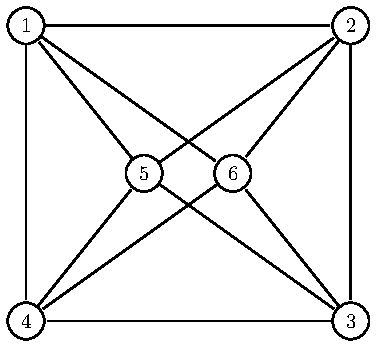
\includegraphics[scale=1]{10_1.pdf} \qquad \qquad
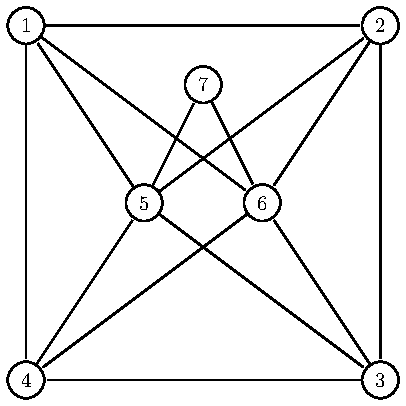
\includegraphics[scale=1]{10_2.pdf}
\end{center}
Here is the first one drawn planar:\\
\begin{center}
	\tikz \graph [nodes={draw, circle}, clockwise] {
		subgraph C_n [V={1,6,4}, radius=4cm] -- subgraph C_n [V={5,2,3}, phase=150, radius=.3cm, nodes={yshift=.25cm}];
		4--5; 1--2; 6--3;
	};
\end{center}


Here is the second one drawn with the $K_5$ subdivision, with subdivided edges highlighted red:\\
\begin{center}
	\tikz \graph [nodes={draw, circle}] {
		subgraph C_n [V={1,2,3,4}, radius=5cm, phase=135, clockwise];
		{[path, --, edges={"red"}, branch right sep=1cm, nodes={xshift=-2cm}] 5,7,6};
		{[induced path, edges={"red"}] 2,3,4};
		6--1--5--2--6--4--5;
	};
\end{center}

\medskip

\item Let $X$ be a set of $n$ points in $\mathbb R^2$ such that the (Euclidean) distance between any pair of distinct points in $X$ is at least 1. Prove that there are at most $3n-6$ pairs of points with distance exactly 1. 

\begin{proof}
	Let $X$ be a set of $n$ points in $\mathbb R^2$ such that the (Euclidean) distance between any pair of distinct points in $X$ is at least 1, and let $G$ be the graph of those points with the edges between points when there are distance 1 apart. BWOC, assume there are more than $3n-6$ edges. This means $G$ is nonplanar, which means there is a $K_5$ or $K_{3,3}$ minor.\\
	There cannot be a $K_5$ minor since if we had a $K_3$ (3 points each dist 1 away), we can center a unit circle at each vertex and the three circles only intersect at 3 points. That means no other vertex could have an edge between all 3.\\
	There cannot be a $K_{3,3}$ for similar reasoning. If we have a vertex adjacent to 3 other vertices, then we can draw a unit circle centered at that vertex. Those 3 vertices are on the circle, and we know that a circle is uniquely defined by 3 points on it, so no other vertex can be adjacent to all three of those vertices.
\end{proof}

\medskip
\item Recall that a graph is outerplanar if it has a plane drawing with all of its vertices touching the outer face.
\begin{enumerate}
\item Let $n \geq 2$. Prove that every $n$-vertex outerplanar graph has at most $2n-3$ edges. 
\begin{proof}
	Let us induct on n\\
	Base case: n=2\\
	This has at most 1 edge ($2n-3$) and is outerplanar.\checkmark \\
	Induction step:\\
	Let $n>2$. Assume the proposition for any outplanar graph with $n'<n$ vertices.\\
	Let $G$ be a $n$-vertex outerplanar graph. Let us remove a vertex, $v$, with degree $\leq$2 (we know one exists from class). By induction hypothesis, $G-v$ has at most $2n-5$ edges. If we add back $v$, we'd be at most adding back 2 edges, so we'd have at most $2n-5+2 = 2n-3$ edges.
\end{proof}
\item Show that part (a) is best possible for all $n\geq 2$ by iteratively constructing graphs $G_2, G_3, G_4, \ldots$ such that $G_n$ is an $n$-vertex, outerplanar graph with $2n-3$ edges.\m
An iterative definition is to take the drawing, and then add a vertex outside of the drawing, connecting it to two vertices that are adjacent by an edge on the outerface.
\begin{center}
	\tikz \graph [nodes={empty nodes, draw, circle}, branch right, grow up] {
		{subgraph P_n [V={1,2}]};
	};\quad
	\tikz \graph [nodes={empty nodes, draw, circle}, branch right, grow up] {
		{subgraph P_n [V={1,2}]} -- {subgraph P_n [V={3}]};
	};\quad
	\tikz \graph [nodes={empty nodes, draw, circle}, branch right, grow up] {
		{subgraph P_n [V={1,2}]} -- {subgraph P_n [V={3,4}]};
		3--2;
	};\quad
	\tikz \graph [nodes={empty nodes, draw, circle}, branch right, grow up] {
		{subgraph P_n [V={1,2}]} -- {subgraph P_n [V={3,4}]} -- {subgraph P_n [V={5}]};
		3--2;
	};\quad
	\tikz \graph [nodes={empty nodes, draw, circle}, branch right, grow up] {
		{subgraph P_n [V={1,2}]} -- {subgraph P_n [V={3,4}]} -- {subgraph P_n [V={5,6}]};
		3--2;
		5--4;
	};
\end{center}
\end{enumerate}

\medskip

\item Let $G$ be an $n$-vertex graph. Suppose for some $t \in \mathbb N$ that $d(u) + d(v) \geq n-t$ for every pair of distinct non-adjacent vertices $u,v \in V(G)$. Prove that the vertices of $G$ can be partitioned into at most $t$ pairwise-disjoint paths.
\begin{proof}
	Let $G$ be an $n$ vertex graph and suppose $\exists t \in \N$ that $d(u) + d(v) \geq n-t$ for every pair of distinct non-adjacent vertices $u,v \in V(G)$. Let us add $t$ vertices that are adjacent to every vertex. Then every vertex's degree goes up by $t$, which will satisfy Ore's condition.  By Ore's theorem, we have that this graph is Hamiltonian. Removing the $t$ vertices add will now make turn the cycle into at most $t$ paths.
\end{proof}
\end{enumerate}

\end{document}
